\documentclass[11pt,a4paper]{article}

% --- Packages ---
\usepackage[utf8]{inputenc}
\usepackage[margin=1in]{geometry}
\usepackage{amsmath}
\usepackage{graphicx}
\usepackage{booktabs}
\usepackage{xcolor}
\usepackage{fancyhdr}
\usepackage[hidelinks]{hyperref}
\usepackage{tikz}
\usepackage{parskip}

% --- TikZ Libraries ---
\usetikzlibrary{shapes.geometric, arrows.meta, positioning, fit, backgrounds}

% --- Theme Colors ---
\definecolor{primary}{RGB}{31, 78, 121}
\definecolor{secondary}{RGB}{0, 130, 115}
\definecolor{accent}{RGB}{196, 82, 36}
\definecolor{darkgray}{RGB}{70, 70, 70}
\definecolor{lightgray}{RGB}{245, 245, 245}

% --- Header & Footer ---
\pagestyle{fancy}
\fancyhf{}
\fancyhead[L]{\bfseries\color{primary} sEMG Acquisition System --- Technical Overview}
\fancyhead[R]{\thepage}
\fancyfoot[C]{\color{darkgray}\footnotesize Single-Channel Module Report}
\renewcommand{\headrulewidth}{0.5pt}
\renewcommand{\footrulewidth}{0.3pt}

% --- Title ---
\title{
  \vspace{-1.5cm}
  {\bfseries\Large\color{primary} Real-Time Surface EMG Acquisition and Monitoring System}\\[6pt]
  {\normalsize\color{darkgray} Technical Overview --- Single Sensor Module}
}
\author{\color{darkgray} Engineering Summary Report}
\date{\today}

\begin{document}

\maketitle
\vspace{-0.5cm}
\noindent\rule{\textwidth}{0.6pt}
\vspace{0.3cm}

\noindent
This report gives a plain-language walkthrough of how the EMG monitoring system works end-to-end, from a muscle contraction picked up by a skin electrode all the way through to a live waveform on screen. It is written as a summary for external review, with an actual recorded dataset included to show the system working in practice.

% ---------------------------------------------------------------------------
\section{How the System Works --- Architecture Overview}

The system is built in three layers that each do a very specific job. The \textbf{Hardware Layer} captures the raw muscle signal. The \textbf{Backend Layer} (running on the host PC) handles all the data processing, filtering, and recording. The \textbf{Frontend Layer} is a browser dashboard that shows everything in real time. Data flows in one direction from hardware all the way to the screen.

\begin{figure}[htbp]
\centering
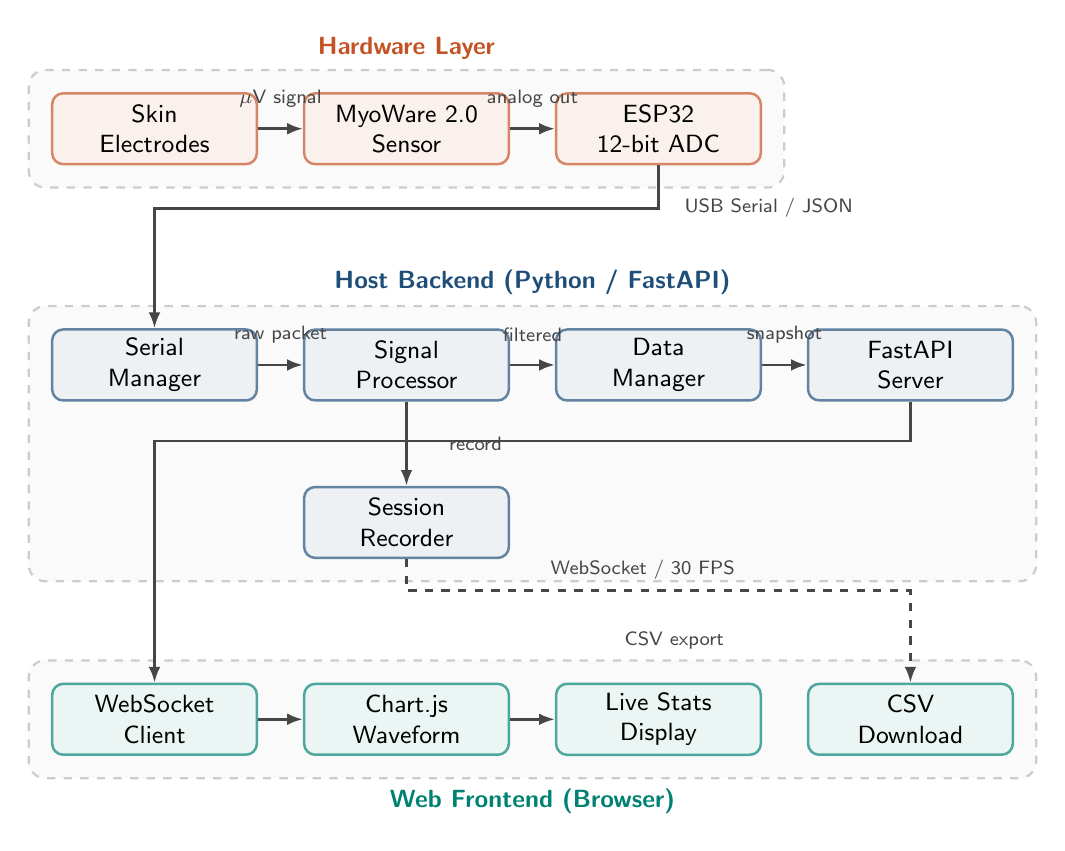
\begin{tikzpicture}[
  every node/.style = {font=\small\sffamily},
  blk/.style = {
    rectangle, rounded corners=4pt,
    draw=#1!70, fill=#1!8,
    minimum width=2.6cm, minimum height=0.9cm,
    align=center, line width=0.9pt
  },
  arr/.style = {-{Latex[length=2mm]}, line width=1pt, draw=darkgray},
  lbl/.style = {font=\scriptsize\sffamily\color{darkgray}, align=center, inner sep=1pt},
  grp/.style = {
    rectangle, rounded corners=6pt,
    draw=gray!40, fill=gray!4,
    dashed, inner sep=8pt, line width=0.8pt
  }
]

% ---- ROW 1: Hardware (y=0) ----
\node[blk=accent]   (skin) at (0,0)     {Skin\\Electrodes};
\node[blk=accent]   (myo)  at (3.2,0)   {MyoWare 2.0\\Sensor};
\node[blk=accent]   (esp)  at (6.4,0)   {ESP32\\12-bit ADC};

% ---- ROW 2: Backend (y=-3) ----
\node[blk=primary]  (ser)  at (0,-3)    {Serial\\Manager};
\node[blk=primary]  (filt) at (3.2,-3)  {Signal\\Processor};
\node[blk=primary]  (dm)   at (6.4,-3)  {Data\\Manager};
\node[blk=primary]  (api)  at (9.6,-3)  {FastAPI\\Server};

% ---- ROW 2b: Recorder (y=-5) ----
\node[blk=primary]  (rec)  at (3.2,-5)  {Session\\Recorder};

% ---- ROW 3: Frontend (y=-7.5) ----
\node[blk=secondary](ws)   at (0,-7.5)  {WebSocket\\Client};
\node[blk=secondary](chart) at (3.2,-7.5){Chart.js\\Waveform};
\node[blk=secondary](stats) at (6.4,-7.5){Live Stats\\Display};
\node[blk=secondary](dl)   at (9.6,-7.5) {CSV\\Download};

% ---- GROUP BOXES ----
\begin{scope}[on background layer]
  \node[grp, fit=(skin)(myo)(esp),
    label={[font=\bfseries\small\sffamily\color{accent}]above:Hardware Layer}] {};
  \node[grp, fit=(ser)(filt)(dm)(api)(rec),
    label={[font=\bfseries\small\sffamily\color{primary}]above:Host Backend (Python / FastAPI)}] {};
  \node[grp, fit=(ws)(chart)(stats)(dl),
    label={[font=\bfseries\small\sffamily\color{secondary}]below:Web Frontend (Browser)}] {};
\end{scope}

% ---- HW ROW: horizontal arrows with midway labels ----
\draw[arr] (skin) -- (myo);
\node[lbl] at (1.6, 0.38) {$\mu$V signal};

\draw[arr] (myo)  -- (esp);
\node[lbl] at (4.8, 0.38) {analog out};

% ---- ESP32 -> SerialManager (bent, label as free node) ----
\draw[arr] (esp.south) -- ++(0,-0.55) -| (ser.north);
\node[lbl] at (7.8, -1.0) {USB Serial / JSON};

% ---- BACKEND ROW: horizontal arrows with midway labels ----
\draw[arr] (ser)  -- (filt);
\node[lbl] at (1.6, -2.62) {raw packet};

\draw[arr] (filt) -- (dm);
\node[lbl] at (4.8, -2.62) {filtered};

\draw[arr] (dm)   -- (api);
\node[lbl] at (8.0, -2.62) {snapshot};

% ---- Recorder branch (vertical, label right side) ----
\draw[arr] (filt.south) -- (rec.north);
\node[lbl, anchor=west] at (3.7, -4.0) {record};

% ---- API -> WebSocket (bent, label as free node) ----
\draw[arr] (api.south) -- ++(0,-0.5) -| (ws.north);
\node[lbl] at (6.2, -5.6) {WebSocket / 30 FPS};

% ---- CSV export: Recorder -> Download (bent, dashed) ----
\draw[arr, dashed] (rec.south) -- ++(0,-0.4) -| (dl.north);
\node[lbl] at (6.6, -6.5) {CSV export};

% ---- FRONTEND ROW: horizontal arrows ----
\draw[arr] (ws)    -- (chart);
\draw[arr] (chart) -- (stats);

\end{tikzpicture}
\caption{End-to-end data flow from muscle contraction to on-screen waveform (single channel).}
\label{fig:arch}
\end{figure}

% --- Hardware Setup Photo ---
\begin{figure}[htbp]
\centering
% -----------------------------------------------------------------------
% REPLACE the gray box below with your actual hardware photo:
%   \includegraphics[width=0.80\textwidth]{hardware_setup.jpg}
% Place the image file (hardware_setup.jpg / .png) in the same folder
% as this .tex file before compiling.
% -----------------------------------------------------------------------
\fbox{\begin{minipage}{0.80\textwidth}\centering\vspace{3.5cm}
  {\large\color{darkgray} [ Hardware Setup Photo ]}\\
  \smallskip
  {\small\color{gray} Replace this placeholder with your actual setup image}\\
  {\small\color{gray} e.g.~\texttt{\textbackslash{}includegraphics[width=0.80\textbackslash{}textwidth]\{hardware\_setup.jpg\}}}
  \vspace{3.5cm}\end{minipage}}
\caption{Physical hardware setup showing the MyoWare 2.0 sensor with surface electrodes placed on the forearm, connected to the ESP32 microcontroller via analog wiring, and interfaced to the host PC over USB.}
\label{fig:hardware}
\end{figure}

\begin{itemize}
  \item \textbf{Hardware Layer} --- Skin electrodes pick up the muscle's electrical activity. The MyoWare 2.0 sensor amplifies this tiny signal so the ESP32 microcontroller can read it. The ESP32 samples the signal 1000 times per second using its onboard ADC (analogue-to-digital converter), then bundles those readings into small JSON messages and sends them over USB to the PC.

  \item \textbf{Backend Layer} --- A Python application running on the PC receives the serial stream. It passes each reading through a digital filter to remove noise (power-line hum, motion artefacts), then computes signal statistics (RMS, peak amplitude) and makes them available to the browser. If a recording session is active, the raw and filtered values are saved simultaneously for later export.

  \item \textbf{Frontend Layer} --- A lightweight HTML dashboard connects to the backend over a WebSocket. It receives data updates 30 times per second and draws rolling waveform charts in real time using Chart.js. The same dashboard lets the user connect/disconnect the device, start and stop recordings, and download CSV files.
\end{itemize}

% ---------------------------------------------------------------------------
\section{The Dashboard Interface}

Figure~\ref{fig:gui} shows the actual monitoring interface running in a web browser. Everything on screen updates live as the hardware is streaming.

\begin{figure}[htbp]
\centering
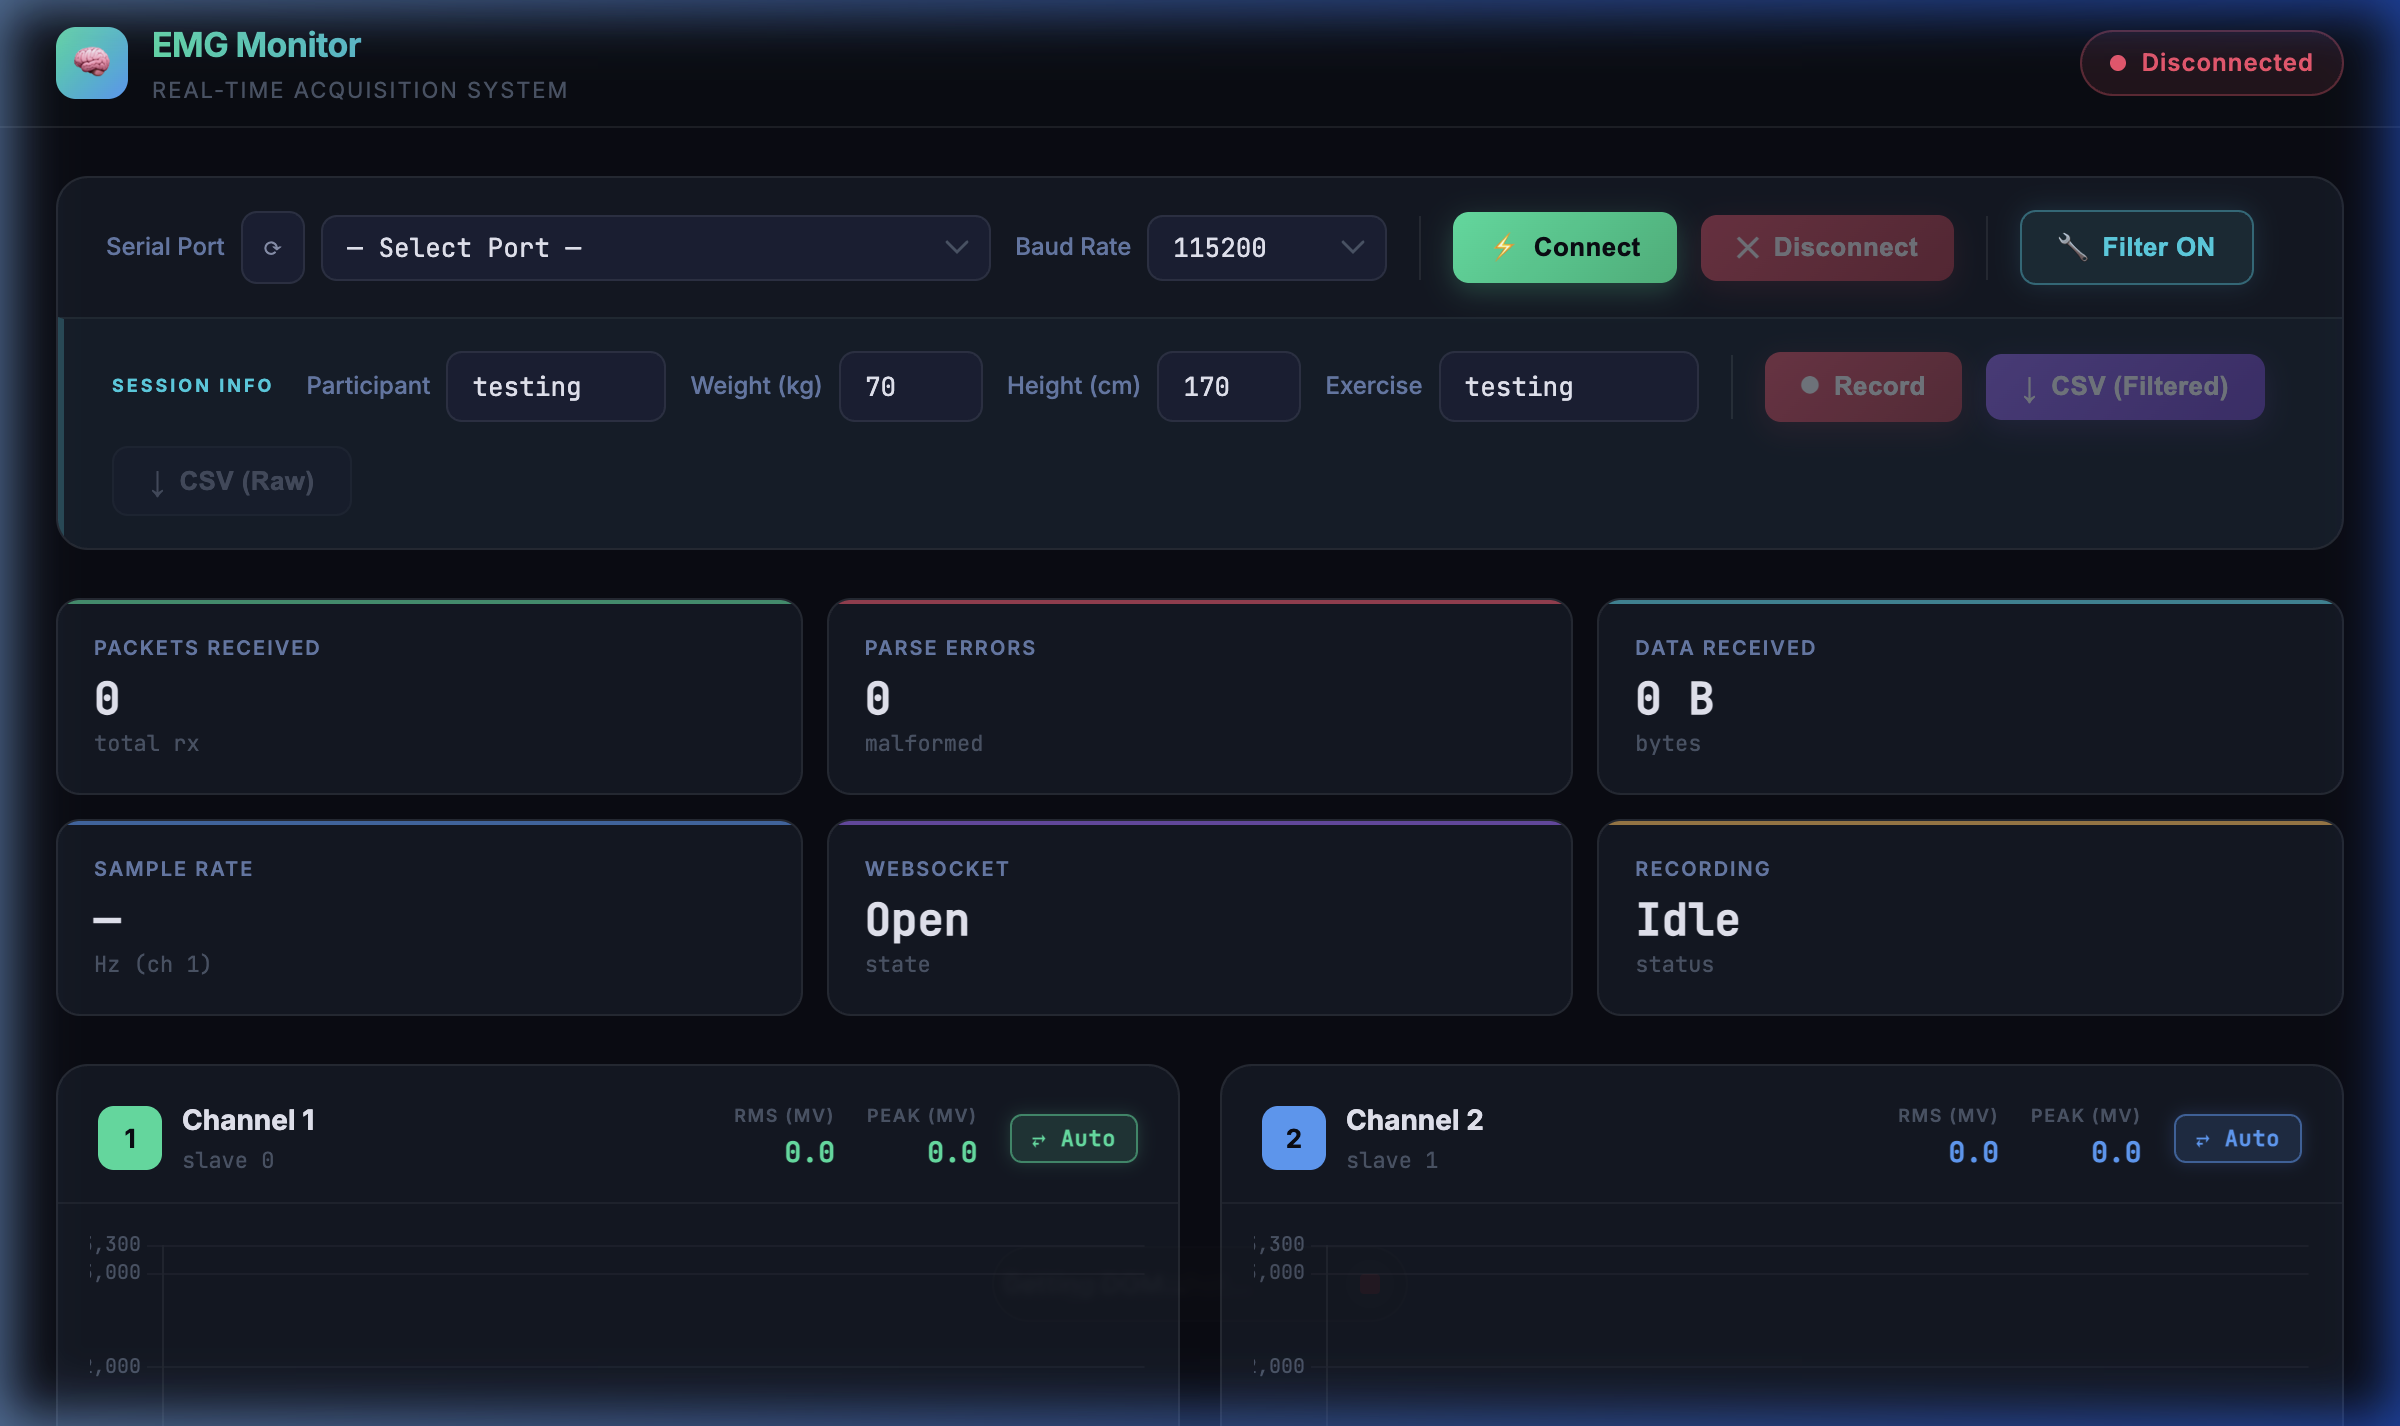
\includegraphics[width=\textwidth]{emg_gui.png}
\caption{The EMG Monitor dashboard showing the device connection controls (top), real-time signal waveforms (centre), and live statistics (RMS, Peak, Peak-to-Peak, sample rate) per channel.}
\label{fig:gui}
\end{figure}

The key controls available to the user are:
\begin{itemize}
  \item \textbf{Port selector} --- scans for connected serial devices and lets you pick the right one with a single click.
  \item \textbf{Live waveforms} --- one chart per channel, scrolling in real time. An ``Auto-scale'' toggle automatically zooms the Y-axis to match the current signal strength.
  \item \textbf{Noise filter toggle} --- switches the digital filter on or off live, so you can instantly see the difference between raw and cleaned signal.
  \item \textbf{Recording controls} --- enter a participant name, exercise label, and body measurements, then hit Start. When the session is done, click Stop and download a ready-to-analyse CSV file.
\end{itemize}

% ---------------------------------------------------------------------------
\section{Signal Cleaning --- Raw vs. Filtered Data}

Raw EMG signals are rarely usable as-is. Two types of noise dominate:
\begin{enumerate}
  \item \textbf{Baseline wander} --- slow drifts caused by breathing, sweat, or electrode movement. Anything below 20\,Hz is rejected.
  \item \textbf{Power-line interference} --- a 50\,Hz hum picked up from nearby electrical equipment. A sharp notch filter removes this without affecting the EMG signal around it.
\end{enumerate}

The backend runs both filters back-to-back on every incoming packet. For real-time display the filter state is carried over between packets so the signal looks continuous with no jumps. When exporting a CSV, a zero-phase version of the same filter is applied to the full recording, which removes any timing shift in the output.

Figure~\ref{fig:plot} shows three complementary views of the same recorded session.

\begin{figure}[htbp]
\centering
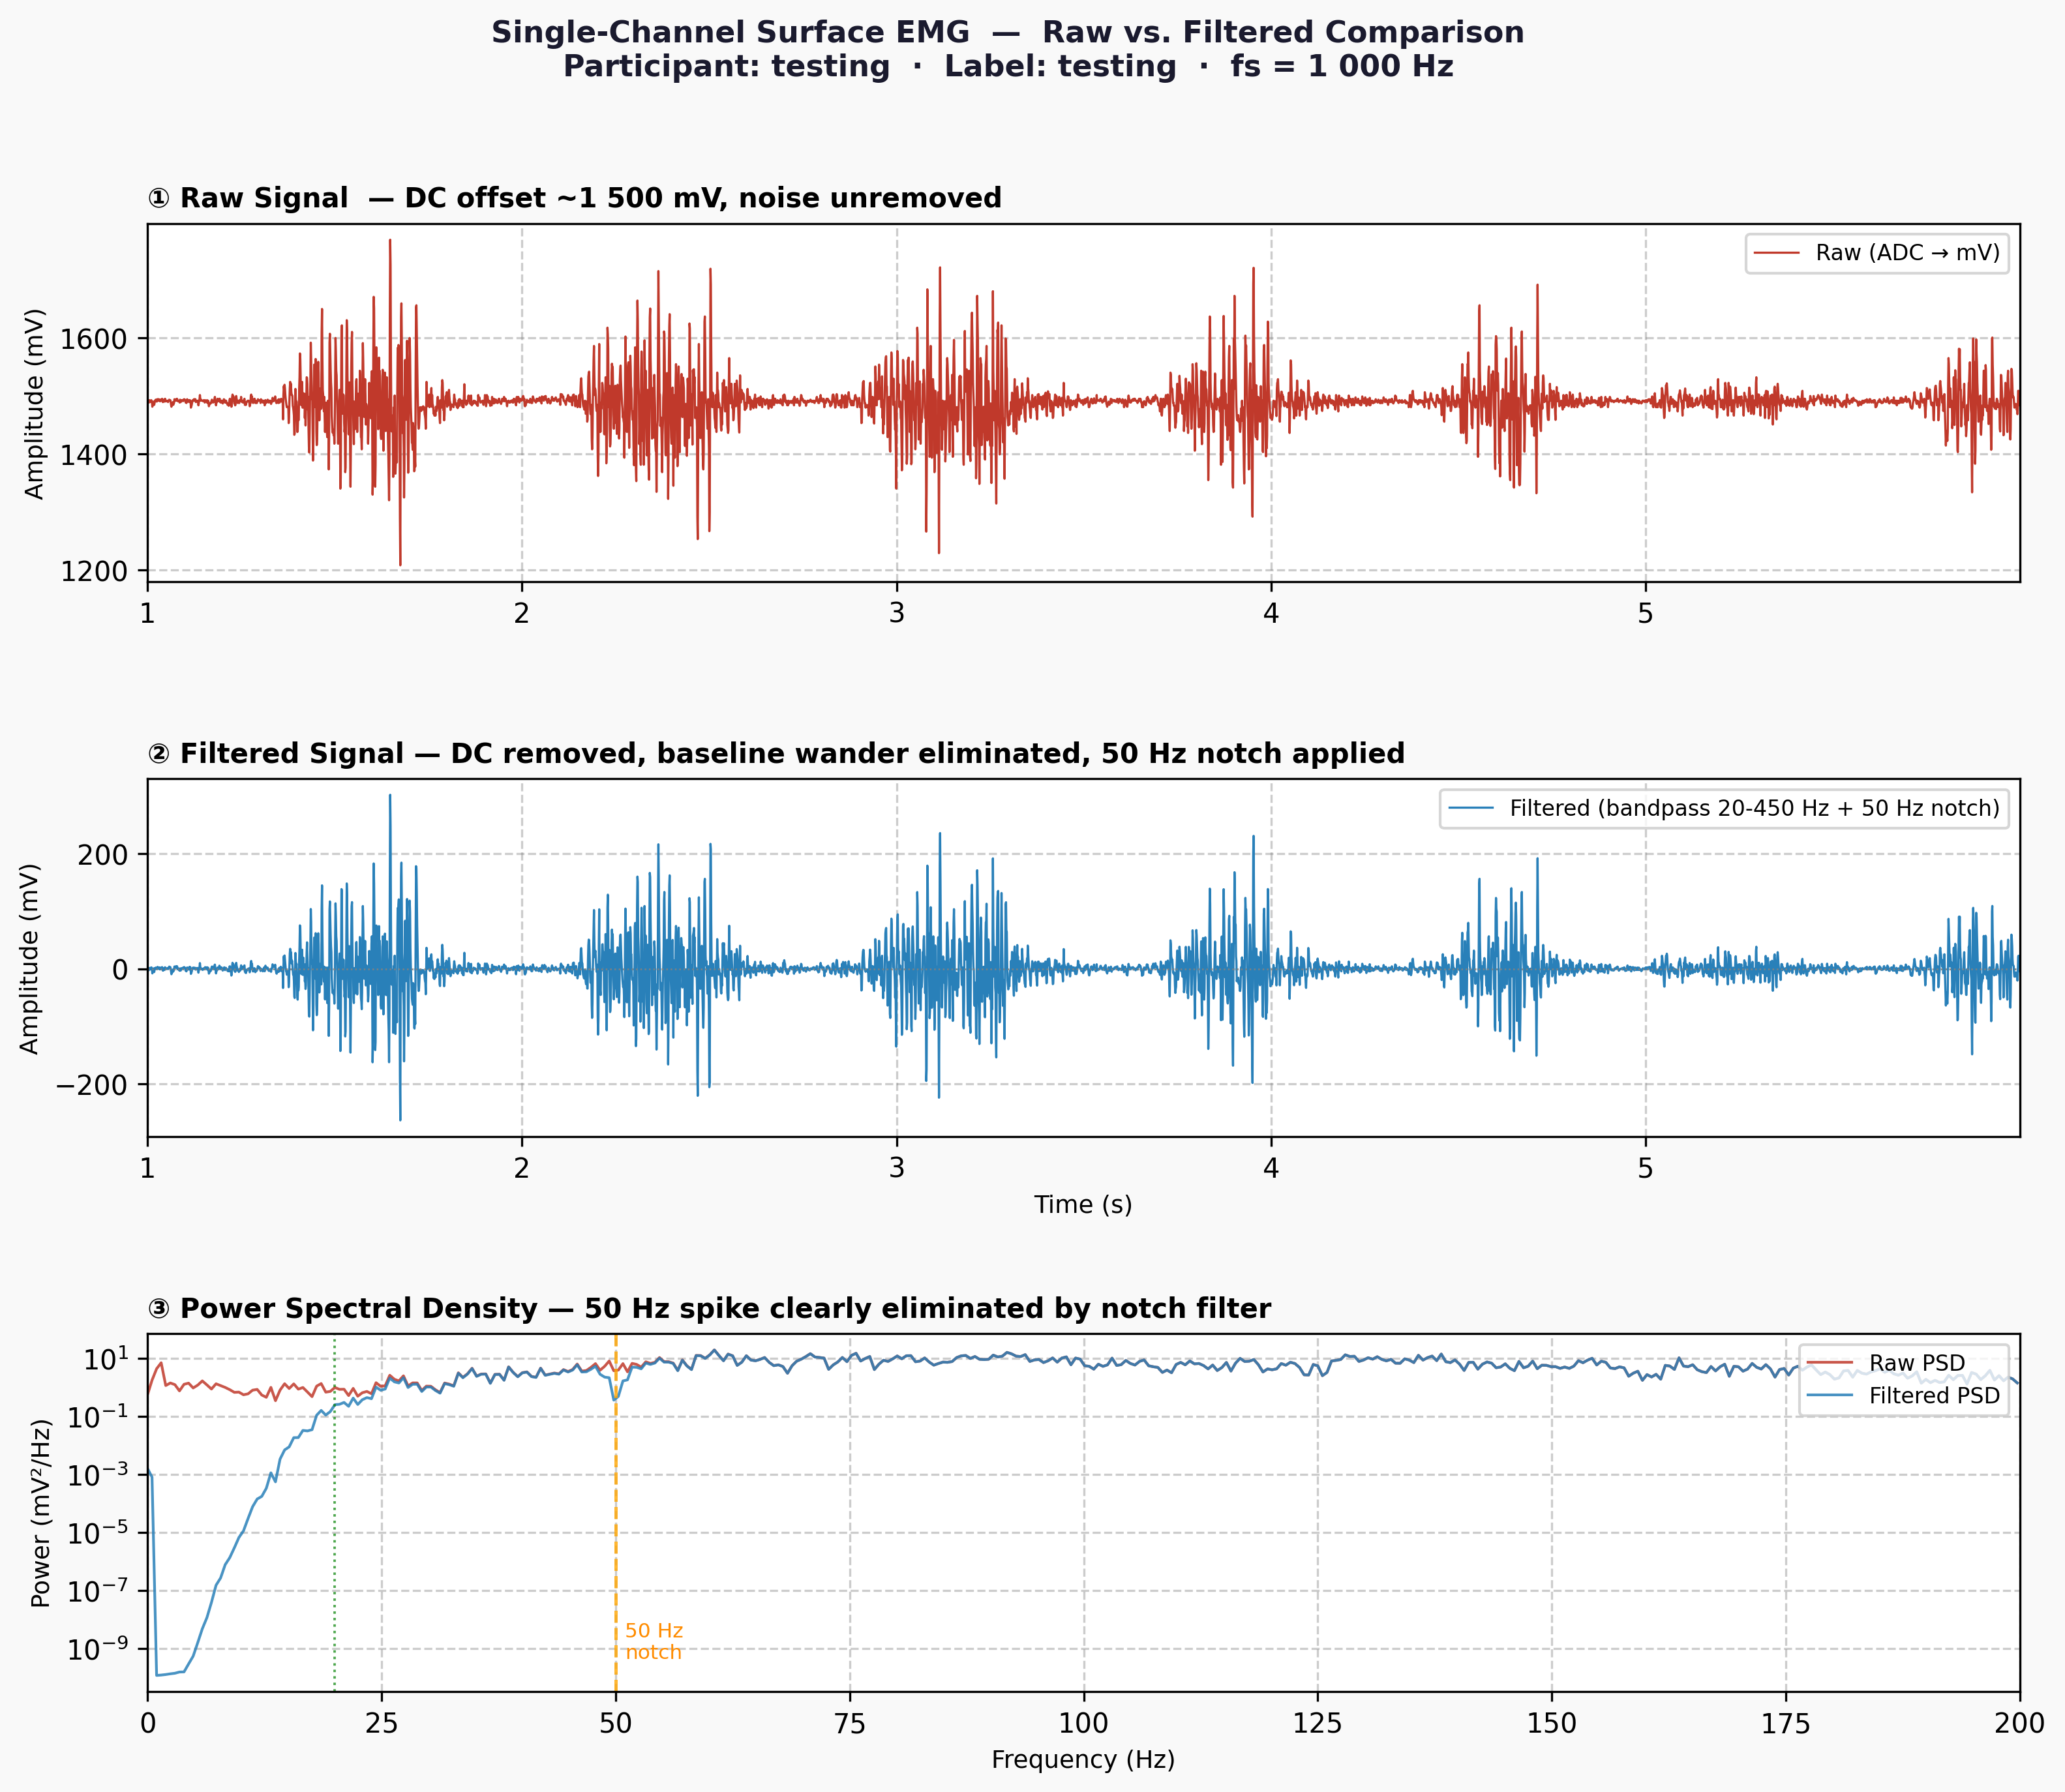
\includegraphics[width=\textwidth]{emg_plot.png}
\caption{Three-panel comparison of a single recorded EMG channel.
  \textbf{Top:} Raw ADC output in millivolts — note the DC bias sitting around 1\,500\,mV (half of the 3.3\,V supply), which has nothing to do with muscle activity.
  \textbf{Middle:} Filtered signal after the 20--450\,Hz bandpass and 50\,Hz notch are applied — the DC is completely removed and the signal is centred at 0\,mV, leaving only genuine muscle activation.
  \textbf{Bottom:} Power Spectral Density (PSD) of both signals up to 200\,Hz. The orange dashed line marks 50\,Hz: the raw signal has a clear power spike there (mains hum), which disappears entirely in the filtered version.}
\label{fig:plot}
\end{figure}

The three panels together make the filtering effect unambiguous. In the time domain (panels 1 and 2) the DC shift alone is dramatic --- 1500\,mV drops to 0\,mV. In the frequency domain (panel 3) the mains-hum spike at 50\,Hz visible in the red raw curve is completely absent from the blue filtered curve. The muscle-activation waveform shape is preserved; only the noise is removed.

% ---------------------------------------------------------------------------
\section{Summary}

This system provides a complete, self-contained pipeline for surface EMG capture and analysis. A muscle contraction that lasts a fraction of a second is picked up by a low-cost wearable sensor, digitised at 1\,kHz, cleaned in real time, displayed live in a browser, and saved to a structured CSV ready for analysis in MATLAB, Python, or any spreadsheet tool. The whole stack runs on a standard laptop with no specialist hardware beyond the sensor module and an ESP32 board.

\noindent\rule{\textwidth}{0.4pt}
{\small\color{darkgray} Data recorded at 1\,kHz using MyoWare 2.0 RAW sensor. Filtering: 4th-order Butterworth bandpass 20--450\,Hz + IIR notch 50\,Hz ($Q=35$). Export format: parallel wide-format CSV with per-sample timestamps.}

\end{document}
